\documentclass[spanish,letterpaper,oneside]{article}
\def\documenttitle {Solución del Sistema 11}
\def\documentsubtitle {Evidencia 2.6: mapa cognitivo de algoritmo}
\def\documentsubject {Eliminación de Gauss-Jordan}
\def\documentauthor {Carlos Mauricio Carvajal Coronado}
\def\coursename {Álgebra Lineal}
\def\coursecode {Evidencia 2.6}
\def\universityname {Universidad Autónoma de Nuevo León}
\def\universityfaculty {Facultad de Agronomía}
\def\universitydepartment {Ingeniero Agrónomo}
\def\universitydepartmentimage {UANL/assets-uanl/logo-uanl.png}
\def\universitydepartmentimagecfg {width=2.1cm}
\def\universitylocation {General Escobedo, Nuevo León, México}
\def\authortable {
  \begin{tabular}{ll}
    Estudiante: & Carlos Mauricio Carvajal Coronado \\
    Matrícula: & 1977875 \\
    Docente: & José de Jesús Miranda Vázquez \\
    Programa: & Ingeniero Agrónomo \\
    Modalidad: & Individual \\
    Evidencia: & 2.6, mapa cognitivo de algoritmo \\
    Fecha: & 22 de octubre de 2026
  \end{tabular}
}
\AddToHook{file/config.tex/after}{\def\stylecitereferences{custom}}
\AddToHook{file/config.tex/after}[aulatex-algebra-lineal]{%
  \def\documentfontsize{12}
  \def\documentinterline{1}
  \def\documentparindent{0}
  \def\documentparskip{5}
  \def\fontdocument{custom}
  \def\fonttypewriter{custom}
  \def\stylecitereferences{custom}
  \def\portraitstyle{style1}
  \def\hfstyle{style1}
  \def\hfwidthwrap{true}
  \def\hfwidthtitle{0.44}
  \def\hfwidthcourse{0.52}
  \def\predocpageromannumber{false}
  \def\pagemarginleft{2.5}
  \def\pagemarginright{2.5}
  \def\pagemargintop{2.5}
  \def\pagemarginbottom{2.5}
  \def\firstpagemargintop{3.8}
  \def\sectionfontsize{\large}
  \def\sectionspacingtop{8}
  \def\sectionspacingbottom{4}
  \def\ssectionfontsize{\normalsize}
  \def\ssectionspacingtop{6}
  \def\ssectionspacingbottom{3}
  \def\defaultimagefolder{UANL/img/}
  \def\usepdfmetadata{false}
}
% Template:     Informe LaTeX
% Documento:    Núcleo del template
% Versión:      DEV
% Codificación: UTF-8
%
% Autor: Pablo Pizarro R.
%        pablo@ppizarror.com
%
% Manual template: [https://latex.ppizarror.com/informe]
% Licencia MIT:    [https://opensource.org/licenses/MIT]

% -----------------------------------------------------------------------------
% CONFIGURACIONES
% -----------------------------------------------------------------------------
% Definiciones previas
\input{src/defs}

% Ajustes usuario
\input{src/config}

% -----------------------------------------------------------------------------
% IMPORTACIÓN DE LIBRERÍAS
% -----------------------------------------------------------------------------
\input{src/env/imports}

% -----------------------------------------------------------------------------
% IMPORTACIÓN DE FUNCIONES Y ENTORNOS
% -----------------------------------------------------------------------------
\input{src/cmd/core}
\input{src/cmd/math}
\input{src/cmd/equation}
\input{src/cmd/image}
\input{src/cmd/title}
\input{src/cmd/other}
\input{src/cmd/column}
\input{src/env/environments}

% -----------------------------------------------------------------------------
% IMPORTACIÓN DE ESTILOS
% -----------------------------------------------------------------------------
\input{src/style/code}
\input{src/style/other}

% -----------------------------------------------------------------------------
% CONFIGURACIÓN INICIAL DEL DOCUMENTO
% -----------------------------------------------------------------------------
\input{src/cfg/init}

% -----------------------------------------------------------------------------
% PORTADA
% -----------------------------------------------------------------------------
\input{src/page/portrait}
\input{src/page/portrait_config}

% -----------------------------------------------------------------------------
% CONFIGURACIÓN DE PÁGINA Y ENCABEZADOS
% -----------------------------------------------------------------------------
\input{src/cfg/page}

% -----------------------------------------------------------------------------
% TABLA DE CONTENIDOS - ÍNDICE
% -----------------------------------------------------------------------------
\input{src/page/index}

% -----------------------------------------------------------------------------
% CONFIGURACIONES FINALES
% -----------------------------------------------------------------------------
\input{src/cfg/final}

\RemoveFromHook{file/config.tex/after}[aulatex-algebra-lineal]


\usepackage[backend=biber,style=apa,natbib=true]{biblatex}
\addbibresource{UANL/ingeniero-agronomo/algebra-lineal/algebra-lineal.bib}
\usepackage{pdflscape}
\usepackage{tikz}
\usetikzlibrary{babel,arrows.meta,positioning}
\definecolor{mapgreen}{RGB}{35,99,71}
\definecolor{mapblue}{RGB}{37,94,136}
\tikzset{
  stepbox/.style={draw=mapgreen,line width=0.7pt,fill=mapgreen!5,
    text width=5cm,minimum height=1.35cm,align=left,inner sep=5pt,font=\small},
  mathbox/.style={draw=mapblue,line width=0.7pt,fill=mapblue!4,
    text width=13cm,minimum height=1.35cm,align=center,inner sep=5pt,font=\small},
  maparrow/.style={-{Stealth[length=2mm]},line width=0.8pt,draw=mapgreen}
}
\pdfcompresslevel=9
\pdfobjcompresslevel=3
\begin{document}
\templatePortrait
\templatePagecfg
\onehalfspacing
\begin{abstractd}
El Sistema 11 de la hoja de problemas de la Evidencia 2 se resuelve mediante
Gauss-Jordan con aritmética racional exacta. La reducción produce
$x=-103/335$, $y=-74/335$ y $z=-379/335$. El determinante $-670$ demuestra
independencia lineal y unicidad. La regla de Cramer y la sustitución en las
tres ecuaciones verifican el resultado. El mapa relaciona cada paso del
procedimiento con su operación matemática, sin añadir unidades o condiciones
físicas que no están especificadas en el enunciado.
\end{abstractd}
\templateIndex
\templateFinalcfg
\section{Introducción}
Los sistemas de ecuaciones lineales describen relaciones simultáneas entre
variables. Una matriz organiza los coeficientes y las operaciones elementales
permiten transformar el sistema sin cambiar sus soluciones
\citep{strang2016}. La reducción por filas permite identificar pivotes,
determinar el rango y distinguir sistemas con solución única, sin solución
o con infinitas soluciones. La comprobación posterior evita confundir una
transformación aritmética incorrecta con una solución del sistema original.

\section{Problema y modelo}
Se selecciona el \textbf{Sistema 11}, situado en la primera página de la
hoja \textit{Problemas evidencia 2 AL AD26} proporcionada por el usuario.
Se mantienen todos sus coeficientes y términos independientes. El problema
pide resolver el sistema asignado mediante uno de los métodos vistos en
clase y presentar el procedimiento en un diagrama tipo algoritmo:
\begin{equation}
\begin{aligned}
-4x+2y+6z&=-6,\\
10x+3y+2z&=-6,\\
-9x-7y+10z&=-7.
\end{aligned}
\end{equation}
Las incógnitas $x,y,z$ pertenecen a $\mathbb R$. El enunciado no especifica
unidades, una aplicación física ni una restricción de no negatividad.

\section{Método e independencia lineal}
Se elige Gauss-Jordan porque produce la matriz identidad y permite leer
directamente las tres incógnitas. El primer pivote puede normalizarse
dividiendo la primera fila entre $-4$. Se emplean
fracciones exactas, sin redondeos intermedios. Las operaciones por renglón
preservan el conjunto de soluciones \citep{strang2016}.

La representación $A\mathbf u=\mathbf b$, con $\mathbf u=(x,y,z)^{\mathsf T}$, es
\[
A=\begin{pmatrix}-4&2&6\\10&3&2\\-9&-7&10\end{pmatrix},\qquad
\mathbf b=\begin{pmatrix}-6\\-6\\-7\end{pmatrix}.
\]
El determinante calculado por cofactores es
\[
\det(A)=-4(30+14)-2(100+18)+6(-70+27)
=-176-236-258=-670\neq0.
\]
Por tanto, las filas de $A$ son linealmente independientes y
$\operatorname{rango}(A)=\operatorname{rango}([A\mid\mathbf b])=3$.
El sistema es compatible determinado: admite una única solución real.

\clearpage
\begin{landscape}
\thispagestyle{empty}
\begin{center}
{\Large\bfseries Mapa cognitivo de algoritmo\par}
\vspace{0.2cm}
\begin{adjustbox}{max totalsize={0.98\linewidth}{0.90\textheight},center}
\begin{tikzpicture}[y=1.5cm,execute at begin node={\setstretch{1}}]
\node[draw=mapgreen,fill=mapgreen,text=white,text width=18cm,align=center,
font=\bfseries\normalsize,inner sep=8pt] (topic) at (7,0)
{Sistema 11: resolución exacta mediante Gauss-Jordan};
\node[font=\bfseries] (ph) at (0,-1) {1. Procedimiento};
\node[font=\bfseries] (mh) at (10,-1) {2. Ejemplo con matemáticas};
\draw[maparrow] (topic.south) -- ++(0,-0.25) -| (ph.north);
\draw[maparrow] (topic.south) -- ++(0,-0.25) -| (mh.north);

\node[stepbox] (p1) at (0,-2.15) {\textbf{1. Escribir la matriz aumentada.} Conservar el orden de incógnitas $x,y,z$ y los signos del Sistema 11.};
\node[mathbox] (m1) at (10,-2.15) {$[A\mid\mathbf b]=
\left[\begin{array}{rrr|r}-4&2&6&-6\\10&3&2&-6\\-9&-7&10&-7\end{array}\right]$.};
\node[stepbox] (p2) at (0,-3.95) {\textbf{2. Normalizar el primer pivote.} Dividir la primera fila entre $-4$.};
\node[mathbox] (m2) at (10,-3.95) {$R_1\leftarrow R_1/(-4)$:
$\left[\begin{array}{rrr|r}1&-1/2&-3/2&3/2\\10&3&2&-6\\-9&-7&10&-7\end{array}\right]$.};
\node[stepbox] (p3) at (0,-5.75) {\textbf{3. Eliminar la primera columna.} Usar el pivote para anular las entradas inferiores.};
\node[mathbox] (m3) at (10,-5.75) {$R_2\leftarrow R_2-10R_1$, $R_3\leftarrow R_3+9R_1$:
$\left[\begin{array}{rrr|r}1&-1/2&-3/2&3/2\\0&8&17&-21\\0&-23/2&-7/2&13/2\end{array}\right]$.};
\node[stepbox] (p4) at (0,-7.55) {\textbf{4. Preparar el segundo pivote.} Dividir la segunda fila entre 8 y multiplicar la tercera por 2.};
\node[mathbox] (m4) at (10,-7.55) {$R_2\leftarrow R_2/8$, $R_3\leftarrow2R_3$:
$\left[\begin{array}{rrr|r}1&-1/2&-3/2&3/2\\0&1&17/8&-21/8\\0&-23&-7&13\end{array}\right]$.};
\node[stepbox] (p5) at (0,-9.35) {\textbf{5. Obtener el tercer pivote.} Eliminar la segunda entrada de la tercera fila y normalizar el resultado.};
\node[mathbox] (m5) at (10,-9.35) {$R_3\leftarrow R_3+23R_2$:
$(0,0,335/8\mid-379/8)$; luego $R_3\leftarrow(8/335)R_3$.\\
$\left[\begin{array}{rrr|r}1&-1/2&-3/2&3/2\\0&1&17/8&-21/8\\0&0&1&-379/335\end{array}\right]$.};
\node[stepbox] (p6) at (0,-11.15) {\textbf{6. Completar la reducción.} Anular las entradas superiores de las columnas tercera y segunda.};
\node[mathbox] (m6) at (10,-11.15) {$R_2\leftarrow R_2-\tfrac{17}{8}R_3$, $R_1\leftarrow R_1+\tfrac32R_3$:
$R_1=(1,-1/2,0\mid-66/335)$, $R_2=(0,1,0\mid-74/335)$.\\
Después $R_1\leftarrow R_1+\tfrac12R_2$:
$\left[\begin{array}{rrr|r}1&0&0&-103/335\\0&1&0&-74/335\\0&0&1&-379/335\end{array}\right]$.};
\node[stepbox] (p7) at (0,-12.95) {\textbf{7. Verificar e interpretar.} Sustituir en las tres ecuaciones originales; comprobar independencia y unicidad.};
\node[mathbox] (m7) at (10,-12.95) {$(-2010,-2010,-2345)/335=(-6,-6,-7)$.\\
$\det(A)=-670\neq0$; solución única:
$(x,y,z)=(-103/335,-74/335,-379/335)$.\\
Sin contexto físico declarado; los valores negativos son válidos en $\mathbb R$.};
\foreach \index in {1,...,7}{\draw[maparrow] (p\index.east) -- (m\index.west);}
\foreach \previous/\next in {1/2,2/3,3/4,4/5,5/6,6/7}{
\draw[maparrow] (p\previous.south) -- (p\next.north);
}
\end{tikzpicture}
\end{adjustbox}
\end{center}
\end{landscape}

\section{Verificación independiente y resultados}
La regla de Cramer proporciona una comprobación independiente de las
operaciones de reducción. Al reemplazar las columnas de $A$ por $\mathbf b$:
\begin{align*}
\Delta_x&=(-6)(44)-2(-60+14)+6(42+21)=206,\\
\Delta_y&=-4(-60+14)-(-6)(100+18)+6(-70-54)=148,\\
\Delta_z&=-4(-21-42)-2(-70-54)+(-6)(-70+27)=758.
\end{align*}
Los cocientes $206/(-670)=-103/335$, $148/(-670)=-74/335$ y
$758/(-670)=-379/335$ coinciden con el mapa. La sustitución exacta comprueba:
\begin{align*}
\frac{412-148-2274}{335}&=\frac{-2010}{335}=-6,\\
\frac{-1030-222-758}{335}&=\frac{-2010}{335}=-6,\\
\frac{927+518-3790}{335}&=\frac{-2345}{335}=-7.
\end{align*}
El residuo $A\mathbf u-\mathbf b$ es el vector cero. Como referencia numérica,
$x\approx-0.307463$, $y\approx-0.220896$ y $z\approx-1.131343$;
las fracciones, no estos redondeos, constituyen la solución exacta.

\section{Interpretación y conclusión}
La solución es la intersección única de los tres planos representados por las
ecuaciones. El determinante no nulo y los tres pivotes confirman que ninguna
ecuación es combinación lineal de las otras. No aparece una fila contradictoria
ni una variable libre: el sistema es compatible determinado.

Los tres valores negativos no invalidan la respuesta, pues el dominio del
ejercicio es real y no se imponen cantidades no negativas. Tampoco deben
interpretarse como dosis, masas o volúmenes: la hoja docente no asigna
significado físico a las incógnitas. Añadir una restricción de no negatividad
alteraría el problema y excluiría la solución encontrada.

Gauss-Jordan determina $(-103/335,-74/335,-379/335)$ y la sustitución confirma
simultáneamente las tres igualdades originales. El mapa vincula las operaciones
con cada matriz resultante y permite seguir el procedimiento sin omitir las
normalizaciones o la eliminación superior. La comprobación independiente
por Cramer respalda la exactitud del resultado.

\printbibliography[heading=bibintoc,title={Referencias}]
\end{document}